\section{Data}
\label{sec:data}
Deze iteratie is er niet veel aangepast aan het database model.
Er is een aanpassing gekomen betreffende de sleutels die gebruikers toegekend krijgen in het systeem voor bijvoorbeeld accountactivatie.

Figuur~\ref{fig:EER diagram} toont het EER-model van de databank. Om overzicht te bewaren worden de attributen die iedere entiteit bezit niet weergegeven in dit model.

\begin{figure}[H]
	\centering
	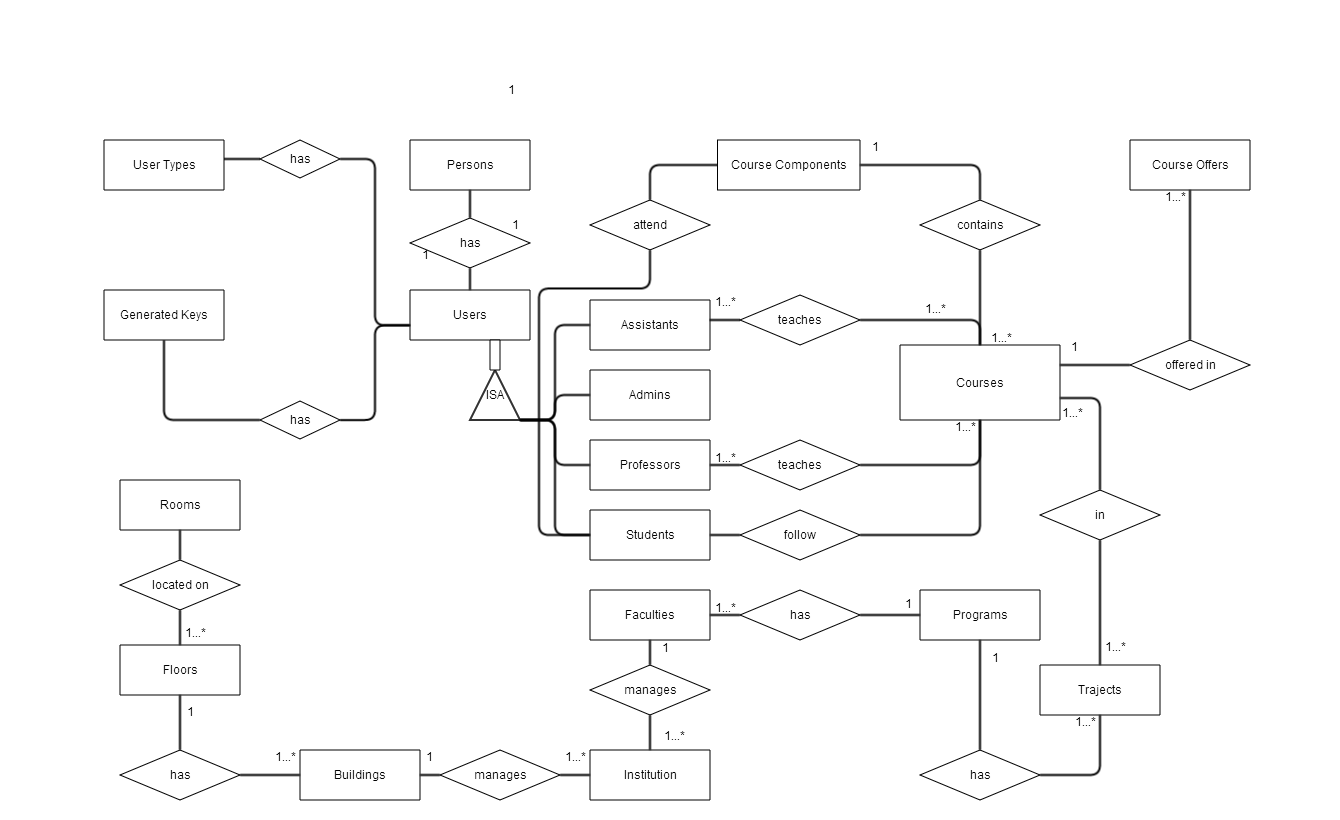
\includegraphics[scale=0.4]{img/ER3-gliffy}
	\caption{EER diagram}
	\label{fig:EER diagram}
\end{figure}

Echter werden wel grote aanpassingen doorgevoerd in het effectieve database schema die dit EER-model verwezenlijkt. 
Er werden tabellen samengevoegd en overbodige tabellen en attributen verwijderd.
Dit gaf een betere integratie met Hibernate.
Figuren \ref{fig:db1}, \ref{fig:db2} en \ref{fig:db3} tonen de huidige status van het database schema.

\begin{figure}[H]
	\centering
	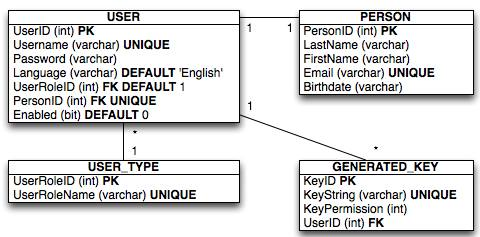
\includegraphics[scale=0.5]{design/EER/schema1}
	\caption{Eerste deel van het database schema}
	\label{fig:db1}
\end{figure}

\begin{figure}[H]
	\centering
	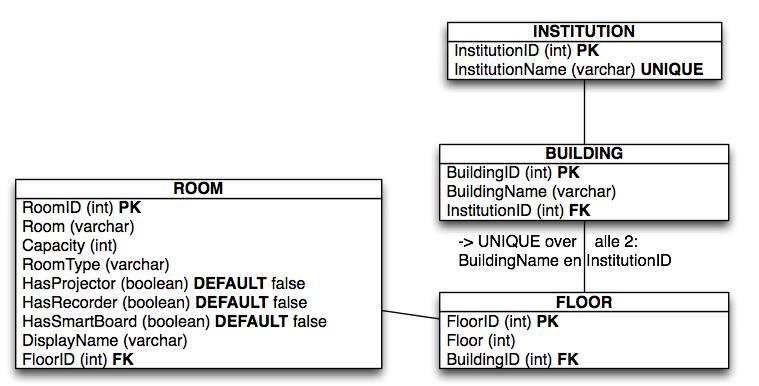
\includegraphics[scale=0.4]{design/EER/schema2}
	\caption{Tweede deel van het database schema}
	\label{fig:db2}
\end{figure}

\begin{figure}[H]
	\centering
	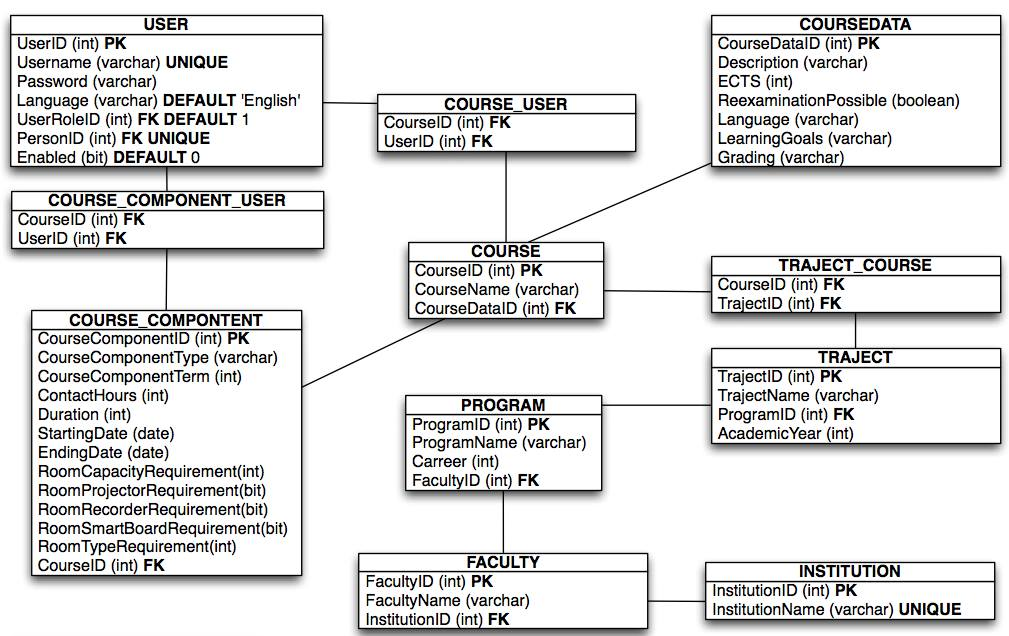
\includegraphics[scale=0.4]{design/EER/schema3}
	\caption{Derde deel van het database schema}
	\label{fig:db3}
\end{figure}